

% \todo{describe part one goal - We involve more theory and prior work research, in following chapters we discuss our case.}
% In the first part of this thesis we focus the comprehensive theory which is needed to absorb in order to interpret results. Not everything is disassembled in detail we go only there where we find something useful for our thesis. This is really based on experience so if the reader is interested only in results used formalism and notation in theory part are important only.

\chapter{Malware analysis} \label{chap:analysis}
Particular goal of this thesis is to create dataset of dynamic malware analysis samples. In this chapter we define basic notions of malware, PE file and malware analysis. We describe sandbox which we use for the analysis and its output. We also address some cyber security challenges and refer to prior arts.


\section{Data cybersecurity challenges}
We address challenges which we found from our point of view and then we refer to the ones listed in \cite{Amit2019}. Authors of that paper also list available datasets for specific kinds of machine learning task in the cybersecurity.

All challenges are based on the complexity of cyber security domain. There are only few industries that are so flexible, dynamic and fast. There are terabytes of data every second in the cybersecurity - cloud, IoT, general network traffic\dots. The supervised machine learning is still the most reliable so we want these data to be labelled. But the detection itself has to be fast because the most significant is ability to detect malware variants (based on similar attributes) and of course zero-day attacks (unseen). Repeated observation might not be possible because modern malware is flexible which could be seen on malware analysis evasion techniques \cite{Afianian2018}. Huge concern is also bias in the data itself caused by multiple things - size, noise, sensibility to small deviations. For instance, if we run several malware samples in sandbox which has access to the internet and malware is able to access its public ip address the bias might be caused by the geographical location of edge router. This is something which could ruin our dataset. Another kind of bias is encryption as mention in the thesis introduction.

Regarding the lack of labeled and certainty in ground truth we can address several problems. If the labelling process is done by human, it become slow and subjective. So the better approach is to develop some heuristic like black lists, white lists or more complex rules, models. That knowledge is little bit more systematic but still not shared which leads us to consensus techniques. This approach is based on combining knowledge from several sources. The goal should be to generalize our detection, but it has another pitfall which are \emph{Advanced Persistent Threats} that are often disposable and unique attack. However, the quality of labelling determines real performance of our future model and its reliable evaluation. Finally, it is sometimes too complex to automate the labelling process, some hope can give us the involvement of unsupervised techniques like anomaly detection or active learning in combination with semisupervised learning.

If we can collect the dataset we should care about its quality. Imbalanced datasets are not speciality of the cybersecurity but it is often presented. The population of specific attacks is not distibuted equally and even the ratio between benign and malicious vary in time. So the balance of our dataset is strongly dependent on the time of data collection. The problem of concept drift is also related to the development over time. It simply addresses the trend of decreasing performance of machine learning models due to the difference of training data in the past and current data. This could be solved by new model or even by ability of adapting existing models in new situations.

% Last remarkable not is many times analyzed statistical assumption
% My
% Data quality, bias, antisandbox detection... where to find samples? (we should definitely mention motivation why we are collecting our own data), public data (this is quite risky to publish in general), everything is fast (zero days), Are those anomalies or malicious?, Imbalanced data sets, encryption everywhere - what to trust..., cryptocurrencies, iot, cloud

% \todo{add some motivation example or latest results... - known malware attacks..}

% Philosophy could be walking around risk management, probability of risk and resulting damage... Maybe more examples of situations where we know how much it cost (Cambridge analytica, ransomware...)
% Maybe something about truth and its protection in the world of lies and fake news
% Confidentiality, integrity and availability

% Use found books or post-hoc go through some articles and formulate the motivation part...

\section{Malware}
Malicious code (also called \emph{Malware}) is code that is intended to disrupt computer, network or its part from functioning. The form or format may vary, it could be JAVA application, microsoft office macro or even pdf file. Malware detection, classification and overall research is part of broader branch of \emph{Intrusion detection} \cite{Cole2009}. Attackers use malware to steal data, use target computer (in C2 or DDOS) or even spy the owner. Malware often gets into target computer via usual communication channels - emails, USB, web download. \cite{KA2018}. Malware may contain more parts which have different role, we call these parts \emph{components}. The software which is not malicious is often called \emph{cleanware}.

Firstly let us clarify several terms. \emph{Malware type} denotes group of malware samples or their components that show same behavior. \emph{Malware family} is collection of malware that has same code base (uses same code components). Example of such family might by \emph{Emotet} which is banking trojan family or CryptoWall which is ransomware family. \emph{Malware variant/strain/version} is malware which is in some existing family but includes new parts which were not earlier detected in this family \cite{Cohen2019}.

Based on specific behavior we can distinguish several fundamental types of malware. Each malware sample may have multiple components and each component may have different type. The most usual malware types follows (their source are \cite{Cole2009, KA2018, Graham2010, Sikorski2012}).

\paragraph{Worm} is malware capable of copying itself in a varieaty of ways and so spreading itself on multiple devices.
\paragraph{Virus} is capable of infecting other executable files by injecting its payload. Infected files are then executed by user.
\paragraph{Trojan} disguises itself as regular program. Their job starts after the user is manipulated. After installation they can steal the data, control target machine\dots
\paragraph{Backdoor} allow attacker access target machine after if their job has succesful ending. The attacker can use multiple machines as botnet controlled by a command and controll server.
\paragraph{Adware} presents unwanted advertisements to user of target machine. They are usually downloaded from the internet.
\paragraph{Information stealer} aims at user's data. Examples are sniffers, grabbers, spyware and key loggers.
\paragraph{Ransomware} locks users out of their computer or encypt their data. It usually threaten the user from not decrypting it before they pay some money.
\paragraph{Rootkit} allow a malware presence concealment.
\paragraph{Dropper} download malicious code or its updates from the internet. The dropper itself is often harmless.
\paragraph{Launcher} is responsible of running malicious code, usually steathly.

According to \cite{AVATLASM39:online} the most seen types on windows are \emph{trojans} and \emph{backdoors}.


% Types, Families
% https://en.wikipedia.org/wiki/Malware
% Find in books!
% https://www.sciencedirect.com/science/article/pii/S1084804519303868 - good overview and taxonomy of malware
\section{File formats}
Malware is defined very generally and it is not limited to specific file format. In general we can find various filetypes. In list below we list some examples.
\begin{enumerate}
  \item Portable executable
  \item Portable Document Format
  \item Microsoft office formats
  \item HTML
  \item Archives
\end{enumerate}

The most see on windows machine are according to \cite{AVATLASM39:online} Portable Executable (PE) files.

\subsection{PE}
The portable executable is file format mainly for executables, object code and DLLs. It is specific for Windows operation system, for 32-bit we use format PE32 and for 64-bit is PE32+. Its complete description is provided by microsoft \cite{PEFormat89:online}. Description of the most important parts follows.

The PE file includes information necessary for Windows operating system (specifically the dynamic linker) to map the file into memory \cite{Gibert2020}. Usual file extensions are \emph{.exe, .dll, .sys}. It consists of two main parts - \emph{Header} and \emph{Sections} (see \ref{fig:pe}). 

\paragraph{Header} contains technical details about the executable. The most important parts are:
\begin{itemize}
  \item DOS header - presented for backward compatibility with older versions of Windows
  \item PE header - executable info such as number of sections, file signature
  \item Optional header - addtional info such as base of data, base of code, address of entry point
  \item Sections table - definition of loading process
  \item Import/export address table - lookup table (pointers) for imported or exported structures (abbrev. \emph{IAT})
\end{itemize}

\paragraph{Sections} contains mainly data and code of the executable. The most important parts are:
\begin{itemize}
  \item code - actual program code (\emph{.text})
  \item imports/exports - \emph{.idata, .edata}
  \item data - static constants (\emph{.data}), variables(\emph{.bss}), other resources (\emph{.rsrc}), debug data (\emph{.rdata})
\end{itemize}

Loading process of PE file starts by parsing the headers and sections table and its validity is checked. The file is mapped into memory according to information in specific header parts. Additional DLLs are loaded into memory based on \emph{IAT}. Finally, file is executed at specified entry point. \footnote{https://github.com/corkami/pics/blob/master/binary/pe101/pe101.png}


\begin{figure}[h]
  \centering
  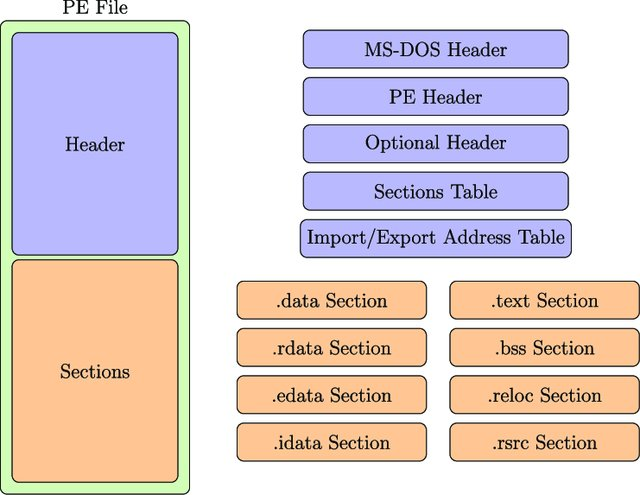
\includegraphics[width=8cm]{figures/pe.jpg}
  \caption{PE file structure (source \cite{Gibert2020})}
  \label{fig:pe}
\end{figure}

\section{Malware analysis}
Malware analysis is process leading to a deeper undertanding of malware features, behavior and overall goal. We can use several techniques and not all of them require execution of examined malware.

Malware analysis is the most relevant at the point where we do not have original source code of malware binary, because its examinantion would often give us much more information. We see the sample as a black box \cite{Sikorski2012}.

After we described malware types we could end up our reasoning as many people before. But the goal of the description of security threats is to be able to respond - prevent further attacks, detect future attacks, identify attacker\dots Authors of \cite{KA2018} summarize our motives in malware analysis in following several reasons. 

We want to find malware components and their role and address its goal. For example we can identify malware consisiting from dropper part which checks running environment and downloading payload from the internet, and from launcher part which is responsible for the payload stealth execution. Another reason might be to understand malware's impact. It is hiding each step and if we do not monitor our systems (for example using integrity checks) we might not realize the threat. We also want to observe and report its behavior in the target computer (filenames, registries\dots) and the network intrusion. The last might be critical for preventing the malware from spreading accross local and global network. Finally, we want to classify the threat and investigate who might be the attacker and what are the motives.

The analysis might be followed by the reaction which often includes antivirus updates - creating new signatures, updating machine learning and other models. The notion of \emph{signature} refers to indicator which is able to detect malicious code on victim machine or even in the network traffic \cite{Sikorski2012}. The signature detection is based on examining outputs of malware analysis and checking specific parts.

We distinguish two basic types of malware analysis - \emph{static} and \emph{dynamic}. In following sections we address each of these and describe their techniques.

\subsection{Static analysis}
By performing this kind of analysis we can exmine target file without executing. Its usage is definitely limited but it can narrow the scope of our interest. \cite{KA2018} Performing the static analysis is usually easier and faster. \cite{Sikorski2012}

\subsubsection{Determining file type}
Earlier in this chapter we listed several file types frequently used by malware. One of initial steps in static analysis is file type determination. The file type might corellate with the file extension e.g. \ \emph{.exe, .sys, .docx}, but reliable technique is file signature examination. This signature is sequence of bytes which is unique across different file types. File signature might be examined manually in some \emph{hex editor}\footnote{example (https://mh-nexus.de/en/hxd/)} or automatically using some programming language or tools\footnote{example https://man7.org/linux/man-pages/man1/file.1.html}. \cite{KA2018} 


\subsubsection{Fingerprinting, comparison}
By fingerprinting is meant generating cryptographic hash value for examined file (e.g. \ \emph{MD5, SHA1}). This hash should give us unique file identifier for future identification. It is used to retrieve known information about malware samples from online sources\footnote{example https://www.virustotal.com/gui/}, where we can find multi anti-virus scans and another useful information. On the other hand we can use special kind of 'hashes' which are able to identify similar malware samples. Those could be fuzzy hashes, import hashes or section hashes \cite{KA2018}.

\subsubsection{String extraction}
Strings are placed in malware file encoded by \emph{ASCII} or other encoding. Their extraction from original binary is valuable tool of the static part of analysis. There might by ip addresses, domain names, file names and other. There are specialized tools for this task \footnote{example http://split-code.com/strings2.html}. Obviously, the challenge in cybersecurity is the imbalance between the attacker and the protector regarding the information about analysis techniques. Which leads us to the file \emph{obfuscation} which is a technique used by attacker to secure strings from extraction. This is often done by \emph{packers} using compression or by \emph{cryptors} by encryption. Of course even such techniques are detectable and vincible using specialized tools.

There are even other techniques e.g. \ \emph{PE header inspection} where we can see imported and exported libraries and functions \cite{Sikorski2012}. Another example is \emphy{Yara rules}, which allow researchers creating indication rules based on textual and binary information of malware sample \cite{KA2018}.

\subsubsection{Code analysis}
Techniques listed above are picking specific feature and by connecting them we might get useful summary as initial hypothesis. But using just executable file we are also able to examine it step by step. We can distinguish \emph{static} and \emph{dynamic} code analysis.

In \emph{static} context we use \emph{disassembler} \footnote{example https://binary.ninja/} which translates machine code back to assembly code which might by further analysed. There is one more sophisticated technique which is also part of \emph{static} contex, it is called \emph{decompilation}. This process translates machine code into higher level programming language such as C or Python \footnote{example https://github.com/avast/retdec}.

In \emph{dynamic} code analyses we use \emph{debugger} to examine translated code during run \cite{KA2018}.

\subsection{Dynamic analysis - sandboxing}
Dymanic analyses techniques allow us examination of running malware sample. The isolated environment for malware execution is often called \emph{Sandbox} (sometimes we call \emph{Sandbox} the application which allow us orchestrate the dynamic analysis process using some interface). During the run we observe the details about malware behaviour and even the reaction of system. In following list we can see different subjects which are often monitored.

\emph{Sandbox} realization is precise work. We need to minimize the risk of malware breaking the border of safe environment. It is usually implemented using virtual machine and \emph{air-gapped} networks (isolated networks) \cite{Sikorski2012}. Using virtual machines is better for overall security of our experiments but there are some significant pitfalls as well. The crucial drawback is that malware might identify suspiciously clean and safe environment and shut down itself before any action. The sandbox setup has to by conscientious to faithfully imitate real environment. We might let some intentional traces of normal usage as mentioned in \cite{CAPESand75:online}. Despite of mentioned facts virtual machine setup is still more frequent than running malware on a pyhsical machine. There are various virtualization software\footnote{examples https://www.virtualbox.org/, https://www.linux-kvm.org/} which provides virtual machines hypervision and user interface (CLI or GUI). Using sophisticated network setup (bridged network adapters, NAT, VPN) we may provide even controlled internet connection (or its simulation). Extracted information from an usual sandbox analysis is listed below and some of them are further dicussed.

\begin{itemize}
  \item Process monitoring - process activity, subprocesses\dots
  \item File system monitoring - dropped files, removed files\dots
  \item Registry keys - read/write operations with windows registry keys including even the read/written data
  \item Network activity monitoring - outgoing and incoming traffic
  \item API calls - external libraries of windows operating system which are called by the malware sample, essentially everything what malware performs should be expressed in the list of api calls
  \item Mutexes - flags which are usually created by process thread to avoid another thread from writing at the same time, they are also used by malware to indicate something (for example its presence to another instance of the same malware)
\end{itemize}

% Let us summarize basics of malware interaction with windows OS (main source \cite{Sikorski2012}). nice to have chapter ANALYZING MALICIOUS
% WINDOWS PROGRAMS

Examples of existing solutions for sandbox environment orchestration are:
\begin{itemize}
  \item CAPEv2 - \url{https://www.capesandbox.com/} (earlier cuckoo sandbox)
  \item ANY.RUN - \url{https://app.any.run/}
  \item Hybrid analysis - \url{https://www.hybrid-analysis.com/}
  \item Joe Sandbox - \url{https://www.joesandbox.com/}
\end{itemize}

\subsection{Sandbox evasion techniques}
As we mentioned earlier creators of malware know how malware might be examined. Malware might delay its execution in order to overcome the timeout of most sandboxes (usually up to half an hour). Malware often checks hardware size, version and other information which could be overlooked during the virtual machine setup and stay generic. It might detect a low number of CPU cores commonly used in sandboxes and other environment details before dropping a payload. If sandbox is running on device with GUI, malware can try user interaction detection \cite{Evolutio45:online}. Comprehensive desription of sandbox evasion techniques can be found in \cite{Afianian2018} and this blog post \cite{Chailytko2019} is describing how we can defeat them.

\section{CAPEv2}
An opensource project called \emph{Cuckoo sandbox} was firstly published in 2011. It started as Google Summer of Code project in 2010 within the Honeynet Project. This project is no more actively developed but in 2019 community developers forked original project\footnote{https://github.com/kevoreilly/CAPEv2} and updated its implementation to python 3. This project is called \emph{CAPEv2} and it is distributed under GPL-3.0 License. There is one publication about original \emph{Cuckoo} sandbox \cite{Oktavianto2013} which is partial source of the following description together with documentation of \emph{CAPEv2} \cite{CAPESand75:online}, other sources are reffered in text.

\emph{CAPEv2} is used to automatically run malicious files, collect results and make some further analysis. It has modular design which allows its integration into more complex infrastructure. Other developers can customize and extend a lot of its functions.
% \todo{nice-to-have image of the interface}

It can analyze various file types (listed below), which can be uploaded using CLI and see results in subdirectory or using a web interface and display results in browser \footnote{public instance https://capesandbox.com/}. List of file types which can be analysed using \emph{CAPEv2} follows:
\begin{itemize}
  \item PE files
  \item DLL files
  \item PDF documents
  \item Microsoft Office documents
  \item URLs and HTML files (even internet explorer context opening some URL)
  \item PHP scripts
  \item CPL files
  \item Visual Basic scripts
  \item ZIP files
  \item Java JAR or applets
  \item Python files 
  \item PowerShell scripts
  \item Microsoft windows installer
  \item Generic binary data such as shellcodes
\end{itemize}


\subsection{Architecture}
\emph{CAPE's} architecture is demonstrated in figure \ref{fig:capearchitecture}. It consists of one or more \emph{cape hosts}, more in case of creating cluster of distributed cape. Each \emph{cape host} might have multiple \emph{analysis guests}. \emph{Cape host} is the environment for sandbox management (file upload, analysis retrieval\dots) usally running Linux distribution\footnote{recommended https://releases.ubuntu.com/20.04/}. \emph{Guests} are virtual machines where particular samples run usually under Windows 7 OS. By default guests are in isolated virtual network where they can not access each other.

\begin{figure}[h]
  \centering
  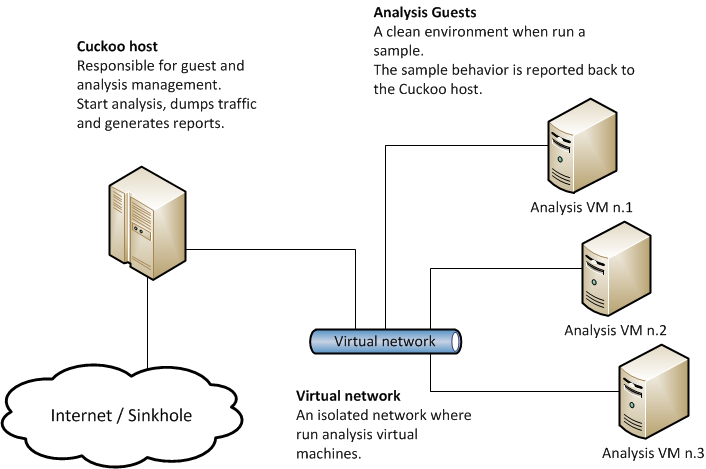
\includegraphics[width=8cm]{figures/architecture.png}
  \caption{Official image of sandbox architecture (source \cite{CAPESand75:online})}
  \label{fig:capearchitecture}
\end{figure}

% \todo{if enough time, we should redraw the image and where we may display even result server and agent.py and capemon.dll, this might be additional image, more low level}

\subsection{Components}
\subsubsection*{Scheduler}
This component continously runs on \emph{host} machine. It check configured limits and proper setup. It manages machinery modules and starts new task if some pends and there is empty \emph{guest} machine. New task is forwarded to \emph{analysis manager}.

\subsubsection*{Analysis manager}
\emph{Analysis manager} is responsible for the whole flow of single task, starts other modules which are parts of analysis and starts\stops machine through \emph{machinery modules}.

\subsubsection*{Auxiliary modules}
Additional modules which are run before analysis or during in \emph{guest} machine. An example of such module is the natwork traffic sniffer which capture network traffic or an screenshot capture tool.

\subsubsection*{Machinary modules}
These modules are used by sandbox to manage virtual machines - start, stop, restore. They are initialized during sandbox start up. Recommended hypervising softwawre for \emph{CAPEv2} is \emph{KVM}.

\subsubsection*{Guest manager}
This component communicates with the \emph{cuckoo agent} and upload sample, checks state of analysis and state of machine. It shutdowns machine in case of timeout.

\subsubsection*{Cape agent}
\emph{Agent} is HTTP server running inside \emph{guest machine} to report its state and allow samples upload and related actions. It has to be started at the same time as machine starts up (added to Windows Startup direction).

\subsubsection*{Analyzer}
Platform-dependent sofware running in \emph{guest} machine which controls the part of flow in the machine. It is started by \emph{agent} and its configuration is provided per analysis. It runs sample using chosen package (specific for each type of uploaded file), if the package is not provided it might be determined automatically. After running target sample it injects it with \emph{cape monitor}.

\subsubsection*{Cape monitor}
DLL which is injected into running sample. It logs any captured behavior using several techniques like hooking functions, following processes, PE dumping It also sends results to the \emph{result server}. \emph{Capemon} is maintained in separate repository\footnote{http://docplayer.net/62887099-Cuckoo-malware-analysis.html}.

\subsubsection*{Result server}
It collects analysis result data and store them.

\subsubsection*{Processing modules}
Processing consists of following parts - processing raw data, signature matching and reporting. First part transforms the raw ouput to readable/searchable format, performs static analysis, extracts network streams. There is structured output at the end. Second part is running particular signatures and collect their results. Signatures are stored in special repository\footnote{https://github.com/kevoreilly/community}. Their interface accepts processed structured data and generates result if current signature matches and realted data. Signature results are added to the structured output. Final part of analysis is reporting, in this part all results are stored in \emph{JSON} report and alsoo in the database (other reporting modules might be added).

List of raw data processing modules follows:
\begin{itemize}
  \item AnalysisInfo - generates some basic information on the current analysis, such as timestamps, version of CAPE and so on.
  \item BehaviorAnalysis - parses the raw behavioral logs and perform some initial transformations and interpretations, including the complete processes tracing, a behavioral summary and a process tree.
  \item Debug - includes errors and the analysis.log generated by the analyzer.
  \item Dropped - includes information on the files dropped by the malware and dumped by CAPE.
  \item Memory - executes Volatility on a full memory dump.
  \item NetworkAnalysis - parses the PCAP file and extracts some network information, such as DNS traffic, domains, IPs, HTTP requests, IRC and SMTP traffic.
  \item ProcMemory - performs analysis of process memory dump. Note: the module is able to process user defined Yara rules from data/yara/memory/index_memory.yar. Just edit this file to add your Yara rules.
  \item StaticAnalysis - performs some static analysis of PE32 files.
  \item Strings - extracts strings from the analyzed binary.
  \item TargetInfo - includes information on the analyzed file, such as hashes.
  \item VirusTotal - searches on VirusTotal for antivirus signatures of the analyzed file. Note: the file is not uploaded on VirusTotal.com, if the file was not previously uploaded on the website no results will be retrieved.
\end{itemize}

\paragraph{Signatures} might isolate some unique behaviour and so identify some malware family or type and spot interesting modification that are performed on the system. Signature does not have only identifier, it also stores description, severity, category, malware family and other related information.

\subsection{Analysis}
An target file upload might be performed using CLI utility of \emph{CAPEv2}, using Web interface, using Python API or using REST API.

In case of a file upload \emph{Capev2} saves it to the database. There is huge amount of options which could be configured for each analysis - used package (for multiple file types), machine to run on, network setup, timeout, priority and multiple addtional options which are presented in original configuration but could be changed per analysis. We can also run only network analysis or only static analysis. Another sandbox component the \emph{Scheduler} keeps track of pending tasks and when there is some free \emph{guest} and pending task, it is run on free machine. The process of execution is managed by \emph{analysis manager}. In case of running new analysis \emph{analysis manager} informs the \emph{result server} where the results are uploaded to. Once running, the analyzer, monitor, configuration and the sample file are uploaded to the \emph{agent}. \emph{Agent} starts the \emph{analyser}, run the sample and injects \emph{monitor} to that. The \emph{analyzer} and \emph{monitor} sends results to the \emph{result server}. After the analysis stops or timeout passed, \emph{analyses manager} stops machine. The collected analysis results are forwarded to \emph{processing modules}. Results are stored in chosen formats and saved to database. \cite{CuckooSa10:online} The whole flow is also described in \ref{fig:capeflow}.

\begin{figure}[h]
  \centering
  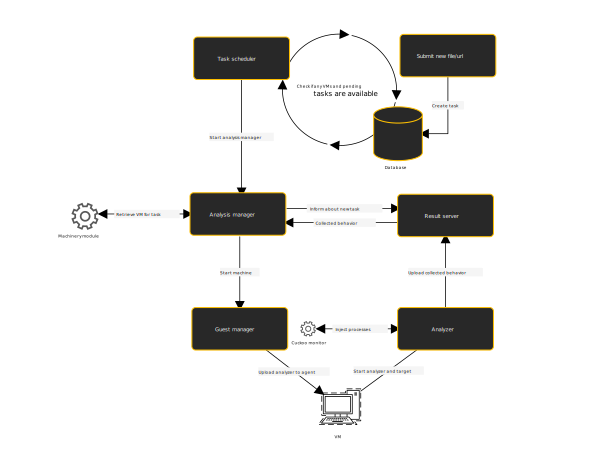
\includegraphics[width=8cm]{figures/flow.svg}
  \caption{Cape components and analysis flow (source \cite{CuckooSa10:online})}
  \label{fig:capeflow}
\end{figure}


\subsection{Network}
\emph{CAPEv2} provides multiple possibilities for \emph{guest} network setup which could be configured per analysis. 

In case of \emph{None} routing, the machine is absolutely isolated, the only traffic is the one with the resuls server. Additionaly, there is \emph{Drop} routing, when the all the traffic is actively dropped (more agresive option). 

Other options provides in some sense internet connection. \emph{Internet} routing is full internet access through specified interface. We can also forward the traffic through another gateway - \emph{VPN}, \emph{SOCKS5} proxy\footnote{example tool https://github.com/RicoVZ/socks5man} or \emph{Tor}\footnote{https://www.torproject.org/}. Last option is to use network simulation like \emph{INetSim}\footnote{https://www.inetsim.org/}.

\subsection{Other}
One of the crucial features of \emph{CAPEv2} is debugger, so we can also perform a non-interactive dynamic code analysis. It allows dynamic anti-evasion bypasses such as \emph{Guloader, Ursnif} or \emph{Zloader} uses.

\emph{CAPE} means \emph{Config And Payload Extraction}. Main motivation behind its creation was malware payload extraction for which it uses techniques like Process injection, Decompression of executable modules in memory or extraction of executable modules. \emph{CAPEv2} automatically creates process dump for each process which is effective to detect basic packers.

\emph{CAPEv2} can detect various malware families such as Emotet, QakBot, Dridex and many others. It also uses Yara rules.


\section{Produced data}
As we stated in the thesis introduction, our goal is to use \emph{behavioural} features from \emph{JSON} reports and \emph{signatures}. In this section we want to demonstrate what we can retrieve from malware analysis tools and refer to some prior art.

absorb chapter data and start of model chapter beginning

\subsubsection{JSON notation} \label{sec:json_notation}
The most comprehensive report which is produced by \emph{CAPEv2} is in \emph{JSON} format. We will use this format as direct input for our model, let us define it here \footnote{documentation https://www.json.org/json-en.html}.

JSON (JavaScript Object Notation) is a most frequently used lightweight data-interchange format. It consists of two essential structures - \emph{collections of key-value pairs} (sometimes called \emph{object}) and \emph{ordered lists}. 
\emph{Object} is unordered list of \emph{key-value} pairs, it is surrounded by curly brackets, pairs are coma-separated and keys are separated by colon from values. \emph{Keys} have to be double-quoted unicode strings. \emph{Values} might be strings, numbers, objects, arrays, boolean or null. \emph{Lists} are surronded by square brackets and contains coma-separated values.

Usually, single \emph{.json} file contains one object, but there are also cases where list of objects is presented.

\subsection{Prior arts}
List of relevant example publications where authors applied machine learning algorithm using the data produced by malware analysis tools.
\subsubsection{Static features}
\begin{itemize}
  \item Strings - \cite{Lee2011}
  \item N-grams (an analysis using bytes subsequences of length $N$ from original binary) - \cite{Fuyong2017}
  \item Entropy of the malware file - \cite{Wojnowicz2018}
  \item Statically extracted API functions calls - \cite{Ahmadi2016}
\end{itemize}

\subsubsection{Dynamic features}
\begin{itemize}
  \item Registry - \cite{Ghiasi2015}
  \item CPU instruction traces - \cite{Carlin2017}
  \item Network traffic - \cite{Boukhtouta2015}
  \item API call traces -  \cite{Galal2015}
\end{itemize}

Other related resources might be in \cite{Singh2020, Sethi2019, Abdessadki2019, Gibert2020}.



%%------------------------------------------
% Nice to have
% https://github.com/kevoreilly/CAPEv2/blob/master/changelog.md
% http://docplayer.net/62887099-Cuckoo-malware-analysis.html
% https://cuckoo-monitor.readthedocs.io/en/latest/hooks.html, more comprehensive description of cape monitor
% Processing modules

% existing solutions and results...
% find basics in books

% api hooking, dumping import reconstruction debugging static parsing - https://www.youtube.com/watch?v=qEwBGGgWgOM

% to appendix we can add also web interface of cuckoo
% \section{Prior}
% works about malware analysis
% works that collected data for machine learning purposes
% Mandlik, Stiborek, everybody who used cuckoo or other sandbox data (reference for what and their results)

% file:///C:/Users/domia/Downloads/Imad-Saiida-IJCNIS-V11-N6-1.pdf
% https://web.archive.org/web/20160418151823/http://www.ijarcsse.com/docs/papers/Volume_3/4_April2013/V3I4-0371.pdf
% https://reader.elsevier.com/reader/sd/pii/S1383762120301442?token=81F1AB06FF0FE40D1B7745234269280FCF2CB0979140E84DB35D6E04A2C622FE6EDA2DE4DA0630E1D73044E3D84A722F&originRegion=eu-west-1&originCreation=20210401090943
% https://iopscience.iop.org/article/10.1088/1742-6596/1140/1/012042/pdf
% file:///C:/Users/domia/Downloads/JCIT4024PPL.pdf
% https://dl.acm.org/doi/abs/10.1145/2046614.2046618?casa_token=MXpfHiylCZcAAAAA:szRMPWfKXTl4wxP2-h32eknCg5dzM2t7RxGjywiJDksmT5FqcUY7pPrIBZchv26HUe3Lwubu5Hru

% file:///C:/Users/domia/Downloads/088851962.pdf

% mention signatures
% usual format which are produced by sandbox and what we can find there
% Reference even docs - no problem, not only books and papers
% Conclusion should be that those data are complicated and their structure also keep some information (order, structure...), that is why we want to focus on structured data and especially json.
% size...


% TODO - nice-to-have
% memory forensics


% If I have to add something - https://publications.sba-research.org/publications/malware_survey.pdf



% mention especially parts which gives more information about the run (mutexes, files, api calls,.. - to be able to reference from data chapter)

% - Summary of potential sorces of metadata
% ○ Abuse.ch - https://bazaar.abuse.ch/api/#api_key
% ○ VirusTotal - https://developers.virustotal.com/v3.0/reference#file-info
% ○ Metadefender - https://onlinehelp.opswat.com/mdcloud/3.1_Retrieving_scan_reports_using_a_data_hash.html
% - Interesting



% Previous connection
% - Nothing before
% Way through this chapter
% - Malware definition and types
% - Malware analysis
% - Challenges
% - Data - input, output...
% - prior
% Next connection
% - We are interested in modeling the data using modern approaches, we know that the data are often structured somehow and that is what we will solve

% - GOALS
%   - Run several instances of CapeV2 sandbox and solve their orchestration for this experiment
%   - Capture behavior of selected malware samples in CapeV2 sandbox and store results
% - Theory part - types, conditions, bias, Malware types, signatures....
% - Sandboxing
% - Previous experiments
% - Our goal in this part
% - Data collection for ML purposes in general


% https://www.groundai.com/project/machine-learning-in-cyber-security-problems-challenges-and-data-sets/1

% https://www.readitquik.com/articles/security-2/cybersecurity-challenges-that-need-to-be-on-your-radar-right-now/